% LaTeX 结构简介
% LaTeX|排版|TeX

本文对 LaTeX 文档的结构做一个简要的介绍. LaTeX 是一种\textbf{所见非所得}的排版语言, 区别于 Word 文档这种\textbf{所见即所得}的排版, 即用户编辑的是代码, 需要经过编译过程才能获得最终的显示效果. 小时物理百科的 PDF 编译使用 \href{https://www.tug.org/texlive/}{TeXlive} 套装中的 XeLaTeX 编译器(\href{https://www.tug.org/texlive/acquire-iso.html}{下载})% 未完成:提供网盘链接
—— 简单来说就是支持中文和其他语言的 LaTeX, 而在线编辑器则是我们自己开发的.

一个简单完整的 LaTeX 文档如下\footnote{LaTeX 文档通常使用 UTF-8 编码的文本文档.}

\begin{lstlisting}[language=latex, caption=test.tex]
\documentclass{article}
\usepackage{amsmath}

\begin{document}
\title{My Title}
\author{My Name}
\maketitle

\section{Introduction}
Some introduction.

\begin{equation}
a^2 + b^2 = c^2 % is this correct?
\end{equation}

\subsection{Subtitle}
Subsection text.

\end{document}
\end{lstlisting}

编译后效果如\autoref{latxIn_fig1}.
\begin{figure}[ht]
\centering
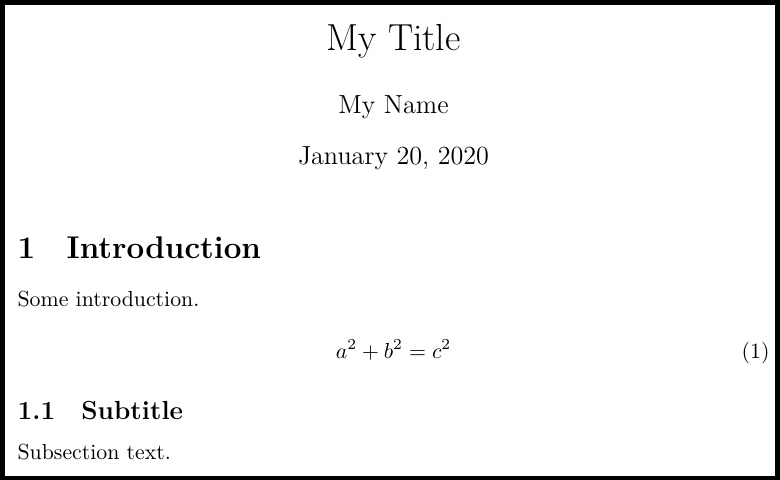
\includegraphics[width=13cm]{./figures/LatxIn_1.png}
\caption{排版效果} \label{latxIn_fig1}
\end{figure}
下面我们来解释本例中的代码.

\subsection{环境}
一个完整的 LaTeX 文档是由许多\textbf{环境}构成的, 环境的格式如下
\begin{lstlisting}[language=latex]
\begin{环境名}[可选设置]
...
...
\end{环境名}
\end{lstlisting}
其中 \verb|[可选设置]| 通常不需要出现. 在一个完整的 LaTeX 文档中, 最大的环境是 \verb|document| 环境(\verb|test.tex| 第 4 行), 文档的所有内容(包括其他环境)都在 \verb|document| 环境中. 在 \verb|document| 环境之前通常会有一些设置, 例如规定文档的类别(第 1 行中的 \verb|article|), 使用一些语言拓展包(即\textbf{宏包}, 如第 2 行的 \verb|amsmath|)等. 这些设置过于复杂, 这里不进行介绍. 一般建议直接直接使用现成的模板.

在 \verb|document| 环境中, 我们可以用 \verb|\section| 和 \verb|\subsection| 等命令把文章划分成不同的章节和子章节. 编译器还可以根据这些命令自动生成目录. 在小时物理百科中, 我们使用四级标题, 分别是\textbf{部分} (\verb|\part|), \textbf{词条} (\verb|\section|), \textbf{节}(\verb|\subsection|), \textbf{子节}(\verb|\subsection|). 注意这些命令只是用于插入对应的标题, 并不构成环境.

另一些常用的环境包括\textbf{公式环境}(第 12 行的 \verb|equation|) 和\textbf{图片环境}(\verb|figure|, 未给出).

\subsection{命令}
LaTeX 中命令的格式为反斜杠 \verb|\| 加连续的大小写字母. 上面的 \verb|\maketitle|, \verb|\begin| 和 \verb|\section| 等都是命令. 有的命令可以单独存在, 而另一些命令需要一个或多个输入, 用花括号表示(如 \verb|\begin{...}| 和 \verb|\section{...}|).

\subsection{注释}
LaTeX 源码中可以用 \verb|% 注释内容| 的格式注释(第 13 行). 注释是给作者看的笔记或批注, 在排版时会被忽略. 如果一行中出现了 \verb|%|, 那么这行剩下的内容都会被视为注释. 如果需要插入百分号而不是注释, 使用 \verb|\%| 即可.

\subsection{多文件编译}
当文档内容较多时(如一本书), 我们可以将主文件中的内容(比如每节)剪切到一个个独立的文件中, 再通过 \verb|\input{文件名}| 命令将这些文档的内容插入主文档中. 例如上面的文档可以划分为两个文件, 主文件 \verb|test.tex| 为
\begin{lstlisting}[language=latex]
\documentclass{article}
\usepackage{amsmath}

\begin{document}
\title{My Title}
\author{My Name}
\maketitle

\input{section1.tex}

\end{document}
\end{lstlisting}

子文件 \verb|section1.tex| 为
\begin{lstlisting}[language=latex]
\section{Introduction}
Some introduction.

\begin{equation}
a^2 + b^2 = c^2 % is this correct?
\end{equation}

\subsection{Subtitle}
Subsection text.
\end{lstlisting}
